% Energi harian turbin: porsi untuk komputer (Raspi vs chip). Angka dari angka.tex (energi_harian.json).
\documentclass[border=4pt]{standalone}
% Gaya bersama gambar deck Demo Day (dipakai semua gambar/*.tex standalone).
\usepackage{amssymb}
\usepackage{fontspec}
\setmainfont{DejaVu Sans Condensed}
\setsansfont{DejaVu Sans Condensed}
\newfontfamily\judulfont{DejaVu Sans}[BoldFont={DejaVu Sans Bold}, Ligatures=TeX]
\usepackage{tikz,pgfplots}
\pgfplotsset{compat=1.18, every axis/.append style={/pgf/number format/assume math mode=true, /pgf/number format/use comma, /pgf/number format/1000 sep={.}}}
\usetikzlibrary{positioning,arrows.meta,calc,shapes.geometric,fit,backgrounds}
\definecolor{gelap}{HTML}{15242B}
\definecolor{teal}{HTML}{285052}
\definecolor{amber}{HTML}{E8A317}
\definecolor{muda}{HTML}{DCE8E8}
\definecolor{abu}{HTML}{8A9499}
\definecolor{teks}{HTML}{1E2B30}
\definecolor{hijau}{HTML}{2F7D5B}
\definecolor{merah}{HTML}{A33A2A}
\color{teks}
\tikzset{
  ubin/.style={fill=muda, rounded corners=5pt, align=center, inner sep=6pt},
  inti/.style={ubin, fill=gelap, text=white},
  panah/.style={-{Stealth[length=3mm]}, line width=1.3pt, draw=amber},
  panahabu/.style={-{Stealth[length=2.5mm]}, line width=1pt, draw=abu},
  judulubin/.style={font=\judulfont\bfseries},
}
% Dibuat otomatis oleh buat_aset.py dari ml/results/energi_harian.json; jangan diedit manual.
\newcommand{\energiTurbin}{270}
\newcommand{\energiQa}{187}
\newcommand{\energiQb}{377}
\newcommand{\hariEnergi}{140}
\newcommand{\raspiWh}{71}
\newcommand{\chipWh}{4,1}
\newcommand{\raspiPersen}{26}
\newcommand{\chipPersen}{1,5}
\newcommand{\raspiPersenA}{19}
\newcommand{\raspiPersenB}{38}
\newcommand{\raspiPersenNum}{26.3}
\newcommand{\chipPersenNum}{1.5}
\newcommand{\hematKwh}{24}
\newcommand{\kaliHemat}{17}
\newcommand{\jRaspi}{182}
\newcommand{\jChip}{10,4}
\newcommand{\periodeEnergi}{2026-03-31--2026-10-20}

\AtBeginDocument{\hyphenpenalty=10000 \exhyphenpenalty=10000}

\begin{document}
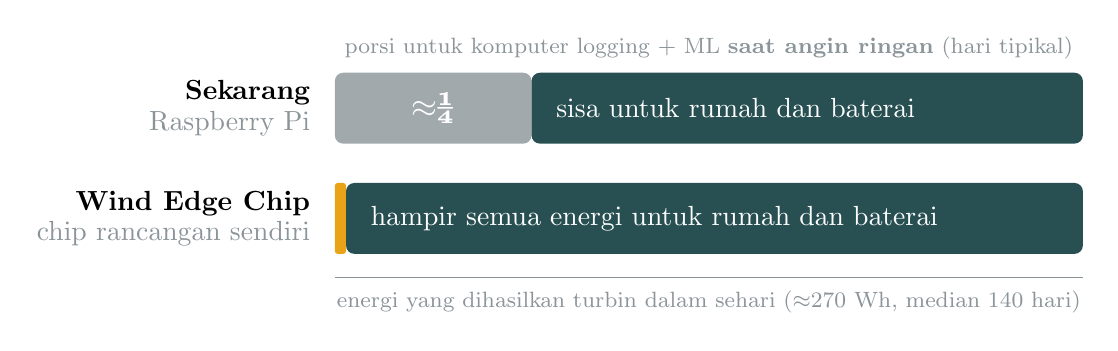
\begin{tikzpicture}[x=0.95cm, y=1cm, font=\fontsize{10}{12}\selectfont]
  \def\L{10}                               % panjang batang = energi turbin per hari
  \pgfmathsetmacro{\r}{\L*\raspiPersenNum/100}
  \pgfmathsetmacro{\c}{max(\L*\chipPersenNum/100, 0.12)}
  % baris 1: sekarang
  \node[anchor=east, align=right, font=\fontsize{10}{12}\selectfont\bfseries] at (-0.2,1.6) {Sekarang\\[-1pt]{\mdseries\color{abu}Raspberry Pi}};
  \fill[abu!80, rounded corners=3pt] (0,1.15) rectangle (\r,2.05);
  \fill[teal, rounded corners=3pt] (\r,1.15) rectangle (\L,2.05);
  \node[text=white, font=\fontsize{12}{14}\selectfont\bfseries] at (\r/2,1.6) {$\approx$\textonequarter};
  \node[text=white, anchor=west] at (\r+0.2,1.6) {sisa untuk rumah dan baterai};
  % baris 2: dengan chip
  \node[anchor=east, align=right, font=\fontsize{10}{12}\selectfont\bfseries] at (-0.2,0.2) {Wind Edge Chip\\[-1pt]{\mdseries\color{abu}chip rancangan sendiri}};
  \fill[amber, rounded corners=1pt] (0,-0.25) rectangle (\c,0.65);
  \fill[teal, rounded corners=3pt] (\c,-0.25) rectangle (\L,0.65);
  \node[text=white, anchor=west] at (\c+0.2,0.2) {hampir semua energi untuk rumah dan baterai};
  % keterangan
  \draw[abu, line width=0.6pt] (0,-0.55) -- (\L,-0.55);
  \node[anchor=north, text=abu, font=\fontsize{8.5}{10}\selectfont] at (\L/2,-0.6) {energi yang dihasilkan turbin dalam sehari ($\approx$\energiTurbin\ Wh, median \hariEnergi\ hari)};
  \node[anchor=south west, text=abu, font=\fontsize{8.5}{10}\selectfont] at (0,2.1) {porsi untuk komputer logging + ML \textbf{saat angin ringan} (hari tipikal)};
\end{tikzpicture}
\end{document}
